\chapter{Neural Networks}

(Artificial) neural networks are a flexible machine learning tool capable of approximating functions with special properties. They can learn from examples, are universal approximators (\href{https://en.wikipedia.org/wiki/Universal_approximation_theorem}{Cybenko's/Universal approximation Theorem}), can deal with noisy and/or incomplete data, and can handle both continuous real and discrete data. Neural networks encompass a wide set of models.

\section{Artificial Neurons}

Artificial neural networks are made up of several \textbf{nodes} (also called artificial neurons or units) connected in a net capable of solving artificial intelligence problems. They are heavily inspired by biological neural networks, down to how the single units work and communicate with each other to learn a certain function.

The main ideas that these models are based on are:

\begin{itemize}
    \item \textbf{Strength reinforcement}: stimuli ``reinforce'' the weights;

    \item \textbf{Plasticity}: the nervous system is highly capable of adapting.
\end{itemize}

Each neuron $i$ has a number of \textbf{inputs} coming from external sources or other units, and corresponding \textbf{weights}, the free parameters that can be modified during the learning phase. Each neuron calculates its \textbf{net input} (weighted sum of inputs) and its output as follows:

\begin{equation*}
    \begin{cases}
        net_i(x) = \sum_j w_{ij} x_j \\
        o_i(x) = f(net_i(x)),
    \end{cases}
\end{equation*}
where $f$ is the unit's \textbf{activator function}.

Note that $w_{ij}$ is the weight of the input coming from the node $j$ and going into the node $i$; some books/libraries/simulators, etc. may use the opposite notation.

\begin{figure}[ht]
    \centering
    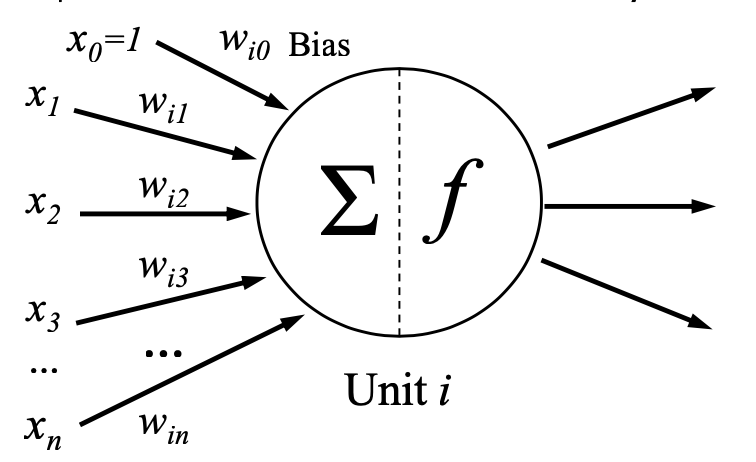
\includegraphics[width=0.5\linewidth]{img/Neuron.png}
\end{figure}

Some examples of activator functions include:

\begin{itemize}
    \item the \textbf{linear activation function};
    \item the \textbf{perceptron/threshold activation function};
    \item the \textbf{sigmoid/logistic function}.
\end{itemize}

\subsection{Perceptrons}

The perceptron was proposed and implemented in 1958 by Frank Rosenblatt. The first perceptron was an actual physical machine designed for image recognition, and not a program. It had a few hundreds of photocells, randomly connected to a layer of neurons.

Multiple perceptrons can be composed and connected to build a network. This is called a \textbf{multi-layer perceptron neural network (MLP NN)}. 

McCulloch and Pitts proposed a neural network model in 1943. In this model, each neuron is in one of two possible states: firing (1), or not firing (0). All synapses (connections) are equivalent and characterized by a weight $w_i$ which is positive for ``excitatory'' connections, and negative for ``inhibitory'' connections. A neuron $i$ becomes active when the sum of the connections coming from other active neurons and the bias is larger than 0. Both inputs and outputs are binary, so it can implement binary classification tasks.

The following pictures illustrate how this model can be used to represent boolean functions AND and OR by using a single neuron. Each neuron has two inputs, plus a bias ($w_0$). Both problems are linearly separable, so if the inputs are represented graphically on a plane, we can draw a single line (described by the net function) that separates all inputs that produce a 0 from all the ones that produce a 1.

\begin{figure}[ht]
    \centering
    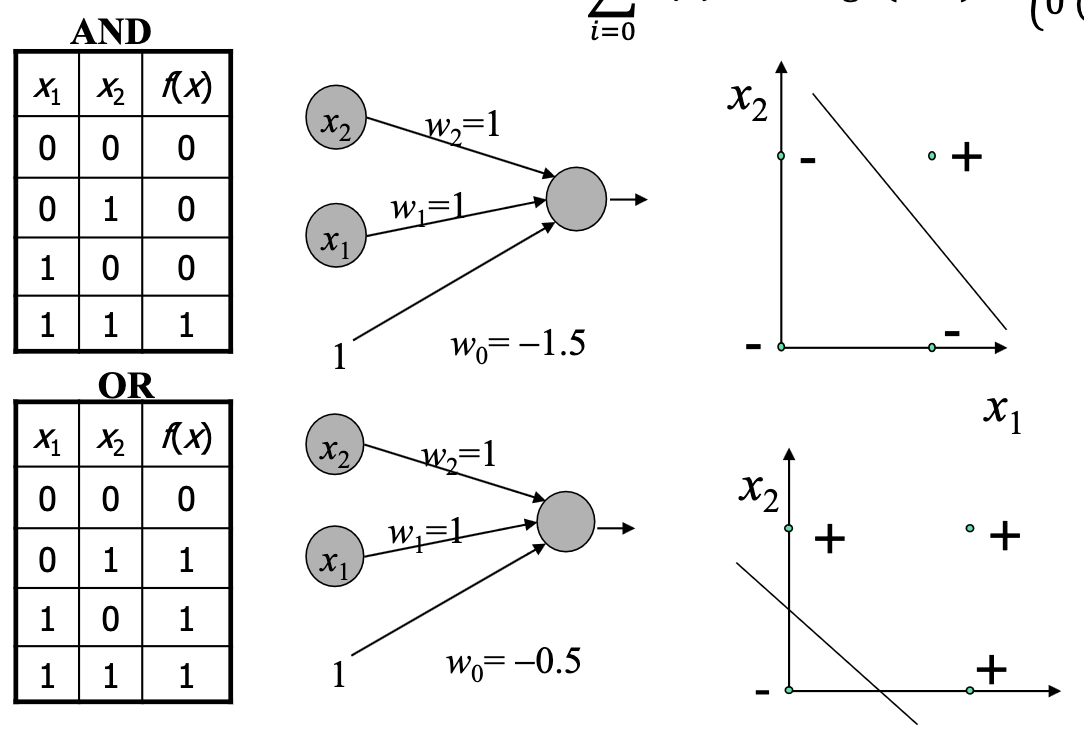
\includegraphics[width=0.5\linewidth]{img/boolean perceptron.png}
\end{figure}

If we instead consider the XOR operator, it corresponds to a non-linearly separable problem, so we can't use a single neuron. The solution is to use a two layer network. The operation can be rewritten as follows:

\begin{equation*}
    x_1 \oplus x_2 = x_1 \cdot \Bar{x_2} + \Bar{x_1} \cdot x_2
\end{equation*}
then we have:
\begin{equation*}
    x_1 \oplus x_2 = \Bar{h_1} \cdot h_2
\end{equation*}
So the XOR operation is moved to a new space that represents the problem as linearly separable:

\begin{figure}[ht]
    \centering
    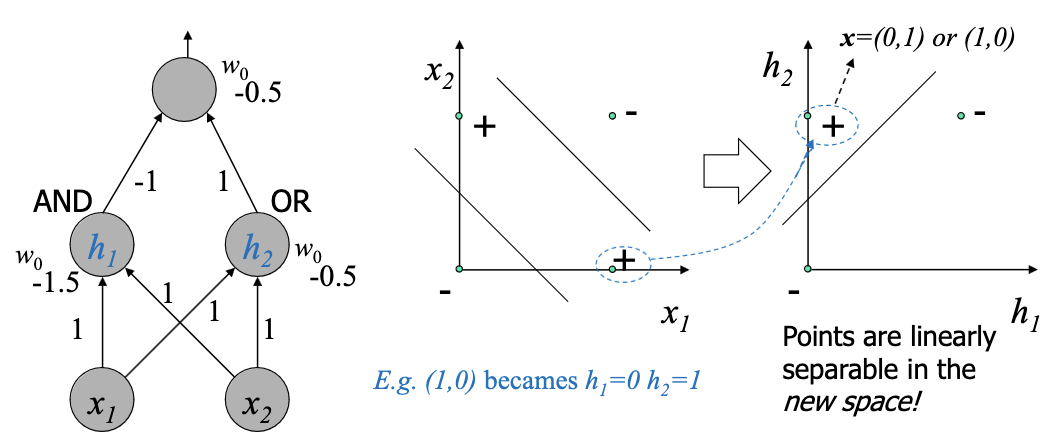
\includegraphics[width=0.5\linewidth]{img/xor perceptron.png}
\end{figure}
This type of composition can be used to perform more complex tasks, extending the network to many layers of abstraction. In NN, this internal representation can be learned.

\section{Learning Algorithms For One Unit Models}

There's two kinds of learning algorithms:
\begin{itemize}
    \item \textbf{Adaline (Adaptive Linear Neuron)}: linear unit during training, can use LMS with either SVD or gradient descent algorithm. This approach an be generalized to multi-level perceptron NNs.

    \item \textbf{Perceptron}: non-linear unit during training, with hard limit or threshold activation function. Can only be used for classification.
\end{itemize}

\subsection{Perceptron Learning Algorithm}

The goal of the algorithm is to minimize the number of misclassified patterns; so it must find $w$ such that $sign(w^Tx)=d$. This is an on-line algorithm, so one step can be done for each input pattern. The algorithm can be summarized as follows:

\begin{enumerate}
    \item Initialize the weights (either to 0 or a small random value);

    \item Pick a learning rate $\eta$;

    \item For each training pattern $<x,d>$, where $d$ is either $+1$ or $-1$, compute $out = sign(w^Tx)$; if $out = d$, don't change the weights, otherwise modify the weights as:
    \begin{equation*}
        w_{new} = w + \eta d x
    \end{equation*}
    or, in a different form,
    \begin{equation*}
        w_{new} = w + \frac{1}{2} \eta (d-out) x
    \end{equation*}
\end{enumerate}

Looking at the problem from a geometrical point of view, it's as if we modified the weight vector $w$ by summing the vector $\eta d x$, where $d$ indicates the direction of the vector with respect to that $x$: if positive, the addition will move $w$ ``towards'' the point, if negative, it will move it ``away'' from it.

The form $w_{new} = w + \eta d x$ is in the form of Hebbian learning, while $w_{new} = w + \eta (d-out) x = w + \eta \delta x$ is in the form of error-correcting learning.

\subsection{Perceptron Convergence Theorem}

``The perceptron is guaranteed to converge (= classify correctly all input patterns) in a finite number of steps if the problem is linearly separable.'' Note that a regressor using LMS does not guarantee convergence.

Let us assume $(x_i, d_i)$ in the TR set, where $d_i \in \{-1,+1\}$. If the problem is linearly separable, here exists $w^*$, solution, such that

\begin{equation*}
    d_i(w^{*T}x_i) \geq \alpha \, , \quad \alpha=\min_i d_i(w^{*T}x_i), \ \alpha > 0
\end{equation*}
hence

\begin{equation*}
    w^{*T}(d_ix_i) \geq \alpha
\end{equation*}
Let us define $x_i' = (d_ix_i)$; then $w^*$ is a solution iff $w^*$ is a solution of $(x_i', +1)$ (it classifies all as positive).  Assuming $w(0) = 0$ at step 0, $\eta = 1$, and $\beta = \max_i\|x_i\|^2$, after $q$ errors (all false negative):

\begin{equation*}
    w(q) = \sum_{j=1}^q x_{(i_j)} \, ,
\end{equation*}
because $w(q) = w(q-1) + x_{i_q}$ according to the update rule used, where $x_{i_j}$ contains the pattern misclassified at the step $j$. Then, we can define the upper and lower bounds for $\|w(q)\|^2$:

\begin{itemize}
    \item the lower bound is given by:
    \begin{align*}
        &w(q) = x_{i_0} + x_{i_1} + \dots + x_{i_q} \\
        &w^{*T}w(q) = w^{*T}x_{i_0} + w^{*T}x_{i_1} + \dots + w^{*T}x_{i_q} \geq q \alpha \ ,
    \end{align*}
    since $w^*$ is the optimal solution.
    With Cauchy-Swartz, it holds that:
    \begin{equation*}
        \|w^{*T}\|^2\|w(q)\|^2 \geq (w^{*T}w(q))^2 \geq (q \alpha)^2
    \end{equation*}
    so
    \begin{equation*}
        \|w(q)\|^2 \geq (q \alpha)^2 / \|w^*\|^2
    \end{equation*}

    \item the upper bound is given by:
    \begin{equation*}
        \|w(q)\|^2 = \|w(q-1) + x_{i_q}\|^2 = \|w(q-1)\|^2 + 2w(q-1)x_{i_q} + \|x_{i_q}\|^2
    \end{equation*}
    where $w(q-1)x_{i_q} < 0$ since it produces a misclassification; therefore
    \begin{equation*}
        \|w(q)\|^2 \leq \|w(q-1)\|^2 + \|x_{i_q}\|^2
    \end{equation*}
    and, by iteration, since $w(0) = 0$:
    \begin{equation*}
        \|w(q)\|^2 \leq \sum_{j=1}^q \|x_{i_j}\|^2 \leq q \beta
    \end{equation*}
    
\end{itemize}
Putting it all together:

\begin{equation*}
    \dfrac{(q \alpha)^2}{\|w^*\|^2} \leq \|w(q)\|^2 \leq q \beta
\end{equation*}
Therefore:
\begin{equation*}
    q \leq \dfrac{\beta}{\alpha^2 / \|w^*\|^2}.
\end{equation*}


\subsection{Differences Between LMS and Perceptron Learning Algorithm}

They are apparently very similar; they both calculate the new value of $w$ by adding a $\delta$ multiplied by the learning rate $\eta$, along with the input $x$ for the Perceptron Learning Algorithm. The $\delta$ for LMS is calculated as $(d - w^Tx)$, while for perceptron learning algorithm it's $(d - sign(w^Tx))$. However similar they are, there a few important differences:

\begin{itemize}
    \item LMS does not necessarily minimize the number of training examples misclassified by the LTU, since it changes the weights for both misclassified and correctly classified ones;

    \item The perceptron learning algorithm always converges for a linear separable problem to a perfect classifier, while LMS has asymptotic convergence (also for non linearly separable problems);

    \item The perceptron learning algorithm is difficult to extend to a NN, while the LMS can be extended to a NN by using the gradient based approach.
\end{itemize}

\section{Activation Functions}

As seen before, the possible activation functions can be a linear function, a threshold function (perceptron/LTU), or a non-linear function such as the \textbf{sigmoidal logistic function}. The latter is a function that assumes a continuous range of values in the bounded interval $[0,1]$. It has the important property of being a smoothed differentiable function. The slope of the sigmoid function is defined by the parameter $a$. Some common examples of functions are:

\begin{itemize}
    \item \textbf{Logistic function}: $f_{\sigma}(x) = \dfrac{1}{1+e^{-ax}}$ (with output in the range $[0,1]$)

    \item \textbf{tanh function}: $f_{tanh}(\frac{x}{2}) = 2f_{\sigma}(x) - 1$ (with output in the range $[-1,+1]$)

    \item \textbf{Radial basis function}: $f(x) = e^{-ax^2}$

    \item \textbf{Rectified linear unit (ReLU)}:
    $f(x) = \begin{cases}
            0 & x < 0 \\
            x & x \geq 0
            \end{cases}$

    \item \textbf{Softplus function}: $f(x) = ln(1+e^x)$
\end{itemize}

The derivative of the identity function is 1. The derivative of the threshold function is not defined, which is why it's not used in LMS. As for sigmoid functions:

\begin{equation*}
    \dfrac{df_{\sigma}(x)}{dx} = f_{\sigma}(x)(1-f_{\sigma}(x)) 
\end{equation*}

\begin{equation*}
    \dfrac{df_{tanh}(x)}{dx} = 1 - f_{tanh}(x)^2
\end{equation*}

\section{LMS With Sigmoidal Function}

Since the sigmoidal logistic function is differentiable, we can derive a LMS algorithm by computing the gradient of the mean square loss function as for the linear units. The output of a neuron is calculated as:
\begin{equation*}
    out(x) = f_{\sigma}(x^Tw)
\end{equation*}
The objective of the algorithm is to find $w = argmin_w E(w) = \sum_p (d_p - out(x_p))^2 = \sum_p (d_p - f_{\sigma}(x_p^Tw))^2$, so the weights that minimize the residual sum of squares.

The gradient descent algorithm is the same, except it uses the new delta rule: $w_{new} = w + \eta \delta_p x_p$, where $\delta_p = (d_p - out(x_p))f'_{\sigma}$. Additionally, the parameter $a$, the slope of the function $f_{\sigma}$, can affect the step of the gradient descent.

Overall: the max of $f'$ corresponds to net inputs close to 0, while the minimum of $f'$ corresponds to \textbf{saturated cases}, as in where the function $f$ goes to either 0 or 1 asymptotically.

\section{Multi Layer Perceptrons}

A MLP can be seen in two possible ways: either as a network of units, or as a flexible function. As a network, a MLP contains a number of units connected by \textbf{weighted links}. The units are organized in layers: the first layer that loads the input is called the \textbf{input layer}; the layer that produces the final output is called the \textbf{output layer}; all other inbetween layers are called \textbf{hidden layers}. The notation used to refer to networks will be the following:

\begin{itemize}
    \item the index $t$ denotes a generic unit, while $k$ denotes an output unit;

    \item the index $u$ denotes a generic input component;

    \item $x$ is a generic input from an external source (if it's an input vector) or from another unit;

    \item if the pattern $x$ is loaded in the input layer, the notation $o$ can be used for both inputs and hidden layer inputs, so, inside the network, the input to each unit $t$ from any source $u$ is simply denoted as $o_u$.
\end{itemize}
As a flexible function, the MLP can be written as a function in the following form:

\begin{equation*}
    h(x) = f_k(\sum_j w_{kj} f_j (\sum_i w_{ji} f_i(\dots))) \, ,
\end{equation*}
where $f_k$ is a sigmoid activation function.

\subsection{Architecture}

The architecture of a NN defines the topology of the connections between units. A \textbf{feedforward architecture} describes a network that operates as follows. For each input pattern $x$, do:

\begin{enumerate}
    \item load the input in the input layer;
    \item compute the output of all the units in the first hidden layer;
    \item compute the output of all the units in the second hidden layer;
    \item ...
    \item compute the output of all the units in the output layer;
    \item compute the error (delta) at the output level.
\end{enumerate}
A \textbf{recurrent architecture} describes a network with feedback loops, which allow the output of units to go ``back'' in the network towards units in previous layers.

\section{Flexibility of NNs}

The hypothesis space of a NN is the continuous space of all the functions that can be represented by assigning the weight values of the given architecture. Depending on the class of values produced as output, the model can deal with both regression and classification tasks, by using, respectively, a linear function or a sigmoidal one. It can also implement multi-regression and multi-class classifiers by defining multiple output units.

When we consider a NN as a function, so in the form
\begin{equation*}
    h(x) = f_k(\sum_j w_{kj} f_j (\sum_i w_{ji} f_i(\dots))) \, ,
\end{equation*}
each $f_j$ can be seen as computed by an independent unit, or a special kind of $\phi$ of Linear Basis Expansion. Additionally, $h(x)$ is non-linear in the parameters $w$. So, we can reformulate the function as follows:
\begin{equation*}
    h(x) = f_k(\sum_j w_{kj} f_j (\sum_i w_{ji} x_i)) = f(\sum_j w_j \phi_j(x,w))
\end{equation*}
The main difference with LBE is that the $\phi$ are adapted to data by fitting the $w$.

\subsection{Theoretical Grounds}

The universal approximation theorem declares that single hidden-layer network (with logistic activation functions) can approximate (arbitrarily well) every continuous function, given enough units; a MLP network can approximate (arbitrarily well) every input-output mapping (provided enough units in the hidden layers), as well. Note that this theorem does not say which learning algorithm to use, nor the number of units needed.

Two issues arise: how can we learn with a NN?, and, how can we decide what NN architecture to use? The answers to these two questions will be provided later. The expressive power of NN is strongly influenced by two aspects: the number of units and the architecture. More specifically, the number of parameters $w$ (which is proportional to the number of units) influences the network capabilities; additionally, even their value can influence the VC-dim of the network: the lower the weights, the lower the VC-dim.

Another important aspect is the number of layers to use in the network. The universal approximation theorem tells us that 1 layer is sufficient to approximate any function, yet it gives no indication on the number of units to use, which may be incredibly high. So, instead of using only one layer, the network is split into multiple layers, each with a limited number of units.

\section{Backpropagation Learning Algorithm}

The learning algorithm used for NN follows the LMS approach. The goal is to adapt the free parameters $w$ in order to obtain the best approximation of the target function. This is normally done by checking the value of the error (or loss) function calculated on the training set. In the case of NNs, however, this is not as straightforward: the network has multiple units across layers, so the learning algorithm must first decide how much credit to give to the hidden units in causing the error to increase.

The so called \textbf{loading problem} is formulated as follows: given a network and a set of examples, is there a set of weights so that the network will be consistent with the examples? The problem is NP-complete, and while networks can in practice be trained in a reasonable amount of time, an optimal solution in not guaranteed.

The idea behind the backpropagation algorithm solution is to extend the gradient descent approach, so it can be used with MLP networks as well. The things we need are:
\begin{itemize}
    \item differentiable loss;
    \item differentiable activation functions;
    \item a network to follow the information flow.
\end{itemize}
What we want to find is $w$ obtained by computing the gradient of the error function. The advantages of the backpropagation algorithm are:
\begin{itemize}
    \item it's easy because of the compositional form of the model;
    \item it keeps track of the quantities local to each unit;
    \item it's efficient, since it's $O(\#W)$ rather than $O(\#W^2)$
    \item supposedly, the brain's learning ``algorithm'' is a local sub optimal approximation of backpropagation (although this debate remains controversial).
\end{itemize}

\subsection{Issues in Training NNs}

The resulting model is often over-parameterized; additionally, the optimization problem is no longer convex, and is potentially unstable.

Some problems in training NNs involve:
\begin{itemize}
    \item \textbf{Hyperparameters}: starting values, choosing between on-line/batch, learning rate, number of hidden units in the network;

    \item \textbf{Multiple minima}: the loss is no longer a simple convex function, so finding a minimum needs specific techniques;

    \item \textbf{Stopping criteria};

    \item \textbf{Overfitting and regularization};

    \item \textbf{Input scaling/output representation}.
\end{itemize}

\subsubsection{Hyperparameters}

\paragraph{Starting values}

The weights are normally initialized with random values near 0; we want to avoid a completely null weight vector, too high values, or all components equal to each other, since these can hamper training. We can also consider the \textbf{fan-in}, i.e., the number of inputs to a hidden unit: $range * 2 /fan-in$. This should be avoided if the fan-in is too large, or if the unit in question is an output unit, since the $\delta$ would be too close to 0 (since we're using backpropagation, those $\delta$ values would be propagated to previous layers, and cause all others to decrease as well).

There's other heuristics, such as a relatively recent one proposed by \href{https://proceedings.mlr.press/v9/glorot10a/glorot10a.pdf}{Glorot and Bengio}.

\paragraph{On-line or Batch gradient descent}

The batch version of the algorithm calculates all the gradients of each pattern over an epoch, then it updates the weights. The stochastic version instead updates the weights after calculating the gradient on one pattern at a time; it also needs a smaller learning rate $\eta$ compared to the batch version, since a value too high may produce a training that's too ``chaotic''.

In terms of MLP with backpropagation, the way the gradient is calculated is:

\begin{equation*}
    - \dfrac{\partial E(w)}{\partial w_{tu}} = - \sum_{p=1}^l \dfrac{\partial E_p(w)}{\partial w_{tu}} = \sum_{p=1}^l \delta_{p,t} o_{p,u}
\end{equation*}
for the batch version, and:
\begin{equation*}
    - \dfrac{\partial E(w)}{\partial w_{tu}} = \delta_{p,t} o_{p,u}
\end{equation*}
for the on-line version.

The batch version produces a more accurate estimation of the gradient, but the on-line version can help avoid local minima while not being as accurate. Additionally, when using the on-line version, a random shuffling of the patterns should be done before each epoch, in order to avoid any bias in the gradient descending.

A variant of the on-line version is the \textbf{minibatch (MB)}. In this version, the epochs are divided in parts; the gradient is summed up to $mb$ patterns ($mb$ = the size of a part) before updating the weights, instead of updating them after every single calculation. Indeed, the batch an on-line versions can be seen as extreme cases of the minibatch: the first uses a part that's exactly the same size as the dataset, the other uses parts of size = 1. A commonly used value of $mb$ is 100, since it's the ideal partitioning of the dataset that exploits GPU memory parallelism the best.

Basic SGD is generally efficient even with NNs, but depends on the number of training data and the number of epochs. There's other heuristic approaches, such as Quick-prop, in which we go to the minima of the local estimated convex function, or R-prop, which does not use the value of the gradient and instead only its' sign.

Some commonly used approaches are \textbf{second order methods}, which calculate more information about the curvature of the objective function in order to plan a better descent. Some methods include approximation of Newton's methods, and Hessian free approaches (conjugate gradients and quasi-Newton methods). These methods, however, have never replaced gradient descent for NN training, because they are susceptible to saddle points (which grow exponentially in high dimensional spaces); gradient descent, instead, shows how to escape saddle points. The length of the training path with gradient descent may still be high for reasons unrelated to local minima or saddle points, however; the reason is still subject of studies. 

In practice, the main basic approaches are more that enough if applied correctly. After all, this optimization is done on the training set, but our focus should be on validation.

\paragraph{Learning rate}

An higher value of $\eta$ causes the descent to be faster but more unstable; a lower value of $\eta$ causes the descent to be slower but more stable. A way to monitor the behavior of the model (and adjust the learning rate as desired) is to plot the \textbf{learning curve}, which is obtained by plotting the error against the number of epochs. Depending on the value of $\eta$, the curve may have a different appearance.

\begin{figure}[ht]
    \centering
    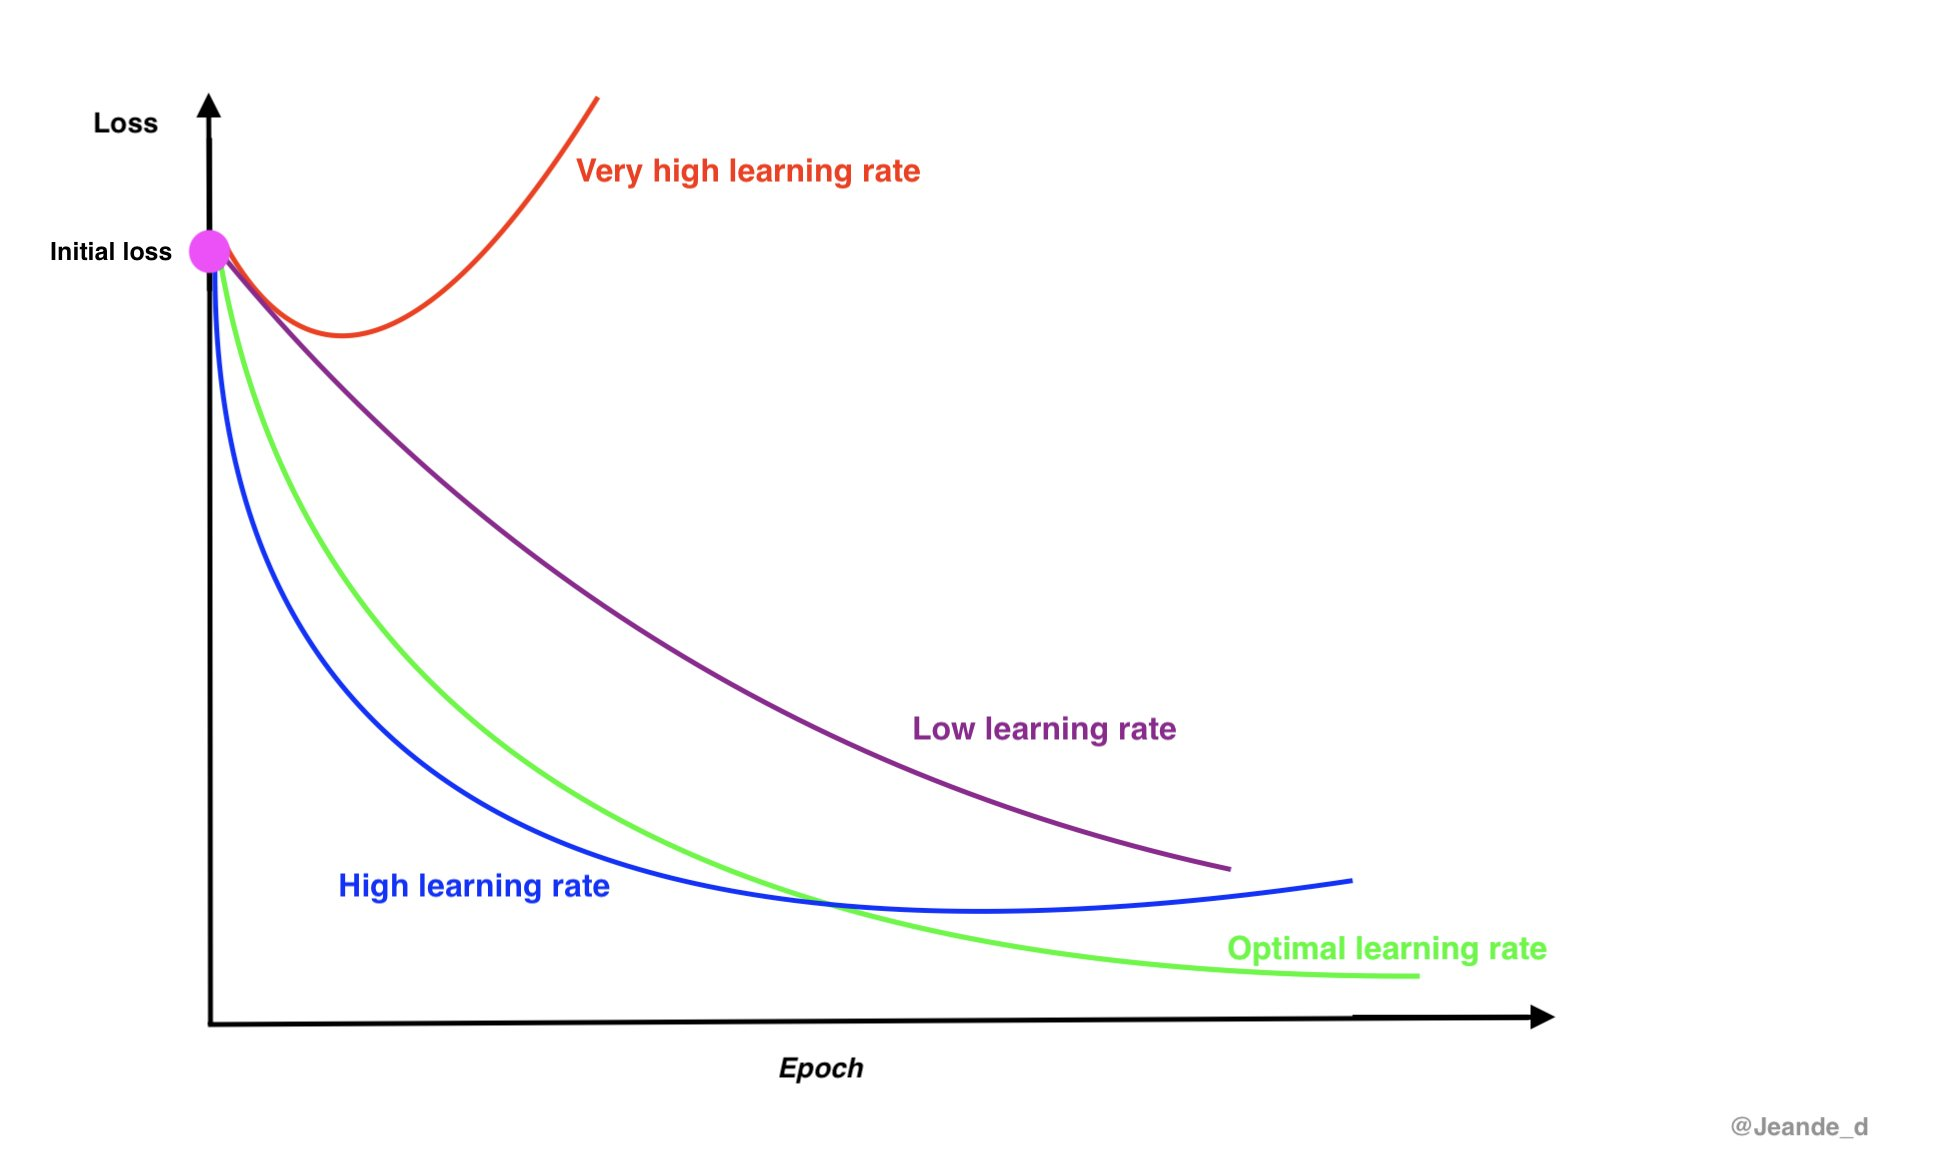
\includegraphics[width=0.5\linewidth]{img/Learning curve and eta.png}
\end{figure}
The green line may appear smooth, but it's actually irregular if we zoom in:
\begin{figure}[ht]
    \centering
    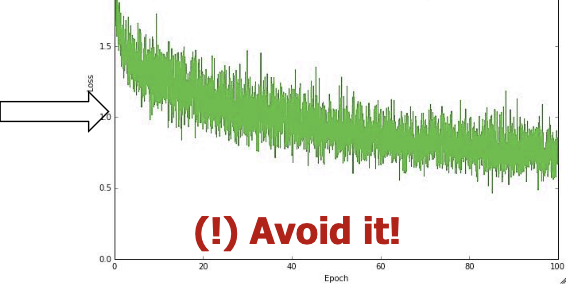
\includegraphics[width=0.5\linewidth]{img/immagine.png}
\end{figure}

In a practical approach, it's useful to consider the mean of the gradients over the epoch, in order to have a uniform approach with respect to the number of input data. When using LMS, dividing by $l$ is equivalent to using $\eta/l$ as our learning rate. As a way to improve the choice of learning rate, the following approaches may be considered:

\begin{itemize}
    \item Using \textbf{momentum}: by adding momentum, $\Delta w$ is now calculated as:
    \begin{equation*}
        \Delta w = - \eta \dfrac{\partial E(w)}{\partial w} + \alpha \Delta w_{old} \, ,
    \end{equation*}
    so we introduce a new term that depends on the previous value of $\Delta w$. $\alpha$ is a value between 0 and 1.

    This is called the ``heavy ball method''. It's faster in plateaus, because the same sign of gradient causes the momentum to increase the delta, and also compensates oscillations in the training, allowing us to use a higher value of $\eta$. It's commonly assumed to help with batch mode more, but can also be used with on-line; in this case, $\Delta w_{old}$ is the $\Delta w_{p-1}$ (as in, of the previous example).

    A variant of momentum is the \textbf{Nesterov momentum}, where the gradient is evaluated after the momentum is applied; so we firs calculate $w = w + \alpha \Delta w_{old}$, the we evaluate the gradient on this new $w$. This variant has been shown to improve the rate of convergence for the batch mode, but not for the stochastic mode.
    
    \item Variable learning rate (start high, then decrease):
    using minibatch, the gradient does not reach 0 even when close to a minimum (as exact gradient can do), hence a fixed learning rate should be avoided. We can linearly decay $\eta$ for each step until iteration $\tau$, using $\alpha = step / \tau$:
    \begin{equation*}
        \eta_s = (1-\alpha)\eta_0 + \alpha \eta_{\tau} 
    \end{equation*}
    and then stop for some iteration, from which we can use a fixed small value of $\eta$. Ideally, the final value of $\eta$ should be $\sim 1\%$ of $\eta_0$, so it takes a few hundred steps to reach it.
    
    \item Adaptive learning rates (changed during training and for each $w$): automatically adapt the learning rate during training, avoiding or reducing the fine tuning phase via hyperparameter selection. Some popular ones include AdaGrad, RMSProp, Adam. Can be combined with momentum.
    
    \item Varying in NNs with many layers (higher for deep layers, or higher for units with few input connections).
\end{itemize}

\paragraph{Number of units}

The number of units controls the complexity of the NN. This choice is in general a model selection issue, so it's selected by a cross-validation. Few units typically lead to underfitting, while too many lead to overfitting, but we can have NNs with many units that don't overfit if regularization is used. We can follow two approaches; either a \textbf{constructive}, incremental, one, in which the learning algorithm decides the (small) starting number of units and then adds more as needed, or a \textbf{pruning} one, where we start with a large network and progressively eliminate weights or units.

A common constructive approach is the \textbf{Cascade Correlation (CC)} learning algorithm. It starts with a minimal network, and adds units until the error is low. It learns both the network weights and topology.

\begin{algorithm}
\caption{Cascade Correlation algorithm.}
\begin{algorithmic}[1]
    \State Start with N0, a network with no hidden units, train it and calculate the error.

    \If{N0 does not solve the problem}
        \State Set i = 1.
        \Repeat 
            \State Create a new unit, and add to the network (creating Ni).
            
            \State Train the unit so that the correlation between the output of the unit and residual error of network Ni-1 is maximized.

            \State Freeze the weights of the unit, and retrain all other units.
            
            \State Calculate error of the new network.
            \State Increase i by 1.
        \Until{Error is $\leq$ a given threshold.}
    \EndIf
\end{algorithmic}
\end{algorithm}
Specifically, this algorithm works by interleaving the minimization of the error function with the maximization of the correlation, which is the covariance of the output of the new unit with the residual error. The role of hidden units is to reduce the residual output error.

\subsubsection{Multiple Minima}

Loss in no longer convex. The function may have multiple minima, as well as maxima. The final result depends a lot on the starting weight values. Ideally, we should try a number of random starting configurations (trials), and then take the mean result (as in, the mean of errors) and check the variance in order to evaluate the model. Then, we can either pick the solution that produces the lowest/median validation error, or we can consider the mean of the outputs.

It's worth noting that finding a local minima with too high error that stops training is not a big issue, since we can always check the final training error (and restart if needed). In general, we don't need to find the global minimum, a ``good'' local minima is sufficient. This is because the minimum we find is of $R_{emp}$, not $R$ (which is what we want to approximate). Also, instead of finding a point corresponding to the null gradient, we may want to stop at a point that has sufficiently small gradient.

Another aspects to consider is that the NN builds a variable size hypothesis space, and tends to increase the VC-dim during training. As the VC-dim increases, the $R_{emp}$ decreases towards the global minimum, but we'll likely incur into overfitting, so stopping before we find the minimum might actually produce a better approximation of the target function.

\subsubsection{Stopping Criteria}

The basic stopping criteria is to check the error (mean or max error $ E$), however, we may not always have enough information to set a tolerance threshold for the error. We may want to use an internal criterion: we stop if the improvement of the error (e.g., less than 0.1\%), or the changes to the weights (e.g. norm of gradient $ < \eta$) are negligible.

We must not stop at an arbitrary number of steps; if it's too small, then it may be too early and cause underfitting, while if it is too large, we may incur into overfitting. Also, if we use K-Fold cross validation, the number of ideal steps for each fold may vary: how do we choose it for the final model, trained over all data? We can consider the number of epochs as a hyperparameter, and select its value as the mean across the folds; however, changing the data size at the end, adding all the records of validation and test set, the stop point may be different, leading to underfitting.

\subsubsection{Overfitting and Regularization}

As said before, we typically don't want the global minimizer of $R_{emp}$, since it would be an overfitting solution. The control of complexity requires some form of regularization (as seen for LBE). This can be achieved by introducing a penalty term, or indirectly by early stopping. Another important step is to perform cross-validation on empirical data to find the best trade-off.

In NNs, learning normally starts by setting the weights to small, random values, and the VC-dim is low. As optimization proceeds, hidden units tend to saturate, increasing the number of free parameters, hence increasing the VC-dim. So, how do we choose when to stop this optimization?

\begin{itemize}
    \item \textbf{Early stopping}: using a validation set to determine when to stop. We ideally want to consider multiple epochs to estimate the error. Since the effective number of parameters grows during the course of training, stopping means limiting the complexity.

    \item \textbf{Regularization}: we can use a regularization related to Tikhonov theory, applied to the loss; a penalty term is added, such that the loss will be calculated as:

    \begin{equation*}
        Loss(w) = \sum_p (d_p - o(x_p))^2 + \lambda\|w\|^2
    \end{equation*}
    This is a form of weight decay, since the new values of the weights during gradient descent will be calculated by adding the term $- \lambda w$, which causes it to decrease even when $\Delta w$ is 0. The regularization parameter $\lambda$ is generally a low value, and is selected in the model selection phase.

    \item \textbf{Pruning methods}: will see later.
\end{itemize}

Remember that, when using regularization, the loss is used during model training, while the error (or risk) for the ``data term'' is used during model evaluation, since it only measures how different the output of the hypothesis is from the correct label. A common misconception is that regularization helps convergence stability, but it does not. It only controls the complexity.

Also, early stopping and regularization can be used together. The difference is that early stopping is an \textbf{empirical approach}, that requires a VL set to decide a stopping point, while regularization is a \textbf{principled approach}, and allows the VL curve to follow the TR curve.

Note, also, that the bias $w_0$ is often omitted from the regularizer, since its inclusion causes the results to not be independent from target shift or scaling. If it's included, it has its own regularization term.

\subsubsection{Putting Momentum and Weight Decay Together}

By putting the two together, the $\Delta w$ can be calculated as:

\begin{equation*}
    \Delta w = -\eta \dfrac{\partial Loss(w)}{\partial w_{tu}} + \alpha \Delta w_{old_{tu}} \doteq \eta \delta_t o_u - \lambda w_{tu} + \alpha \Delta w_{old_{tu}}
\end{equation*}
Here, the index $p$ is omitted and we consider the Loss as the sum of Error + Penalty and using $\eta$ only for the Error term. This form, where $\Delta w$ includes $\lambda$, $\eta$ and $\alpha$, is often used by major tools/libraries for NNs. However, we can define a form that keeps the hyperparameters separated, b y writing:

\begin{equation*}
    \Delta w = \eta \delta_t o_u + \alpha \Delta w_{old_{tu}} \, ,
\end{equation*}

\begin{equation*}
    w_{new_{tu}} = w_{tu} + \Delta w_{tu} - \lambda w_{tu} 
\end{equation*}
In this form, eta and alpha are independent.

\subsubsection{Input Scaling/Output Representation}

Preprocessing of the data can have a large effect on the result of training. Data should be normalized via either standardization (each feature is modified so that mean is 0 and standard deviation is 1), or rescaling (the range of values is restricted to [0,1]).

For regression, there's one or more output linear units; for classification, there's either a singular binary output unit, or there's multiple binary units. In the latter case, we can use a sigmoid to choose the threshold to assign the class, a rejection zone, or 1-to-K encoding to choose the ``winner'' class. Often, the symmetric logistic function learns faster. To avoid asymptotic convergence, 0.9 and 0.1 can be used instead of 1 an 0 as a label value (for the logistic function, for the tanh function -0.9 is used instead of -1). In any case, the target range must be in the output range of units. If targets are 0/1, it's common to use the Softmax function:

\begin{equation*}
    o_k(x) = \dfrac{e^{(-net_k)}}{\sum_{j=1}^Ke^{(-net_j)}}
\end{equation*}
We can also use an alternative error/cost function, where we minimize the cross entropy:

\begin{equation*}
   E(w) = - \sum_{i \in TR} \{ d_i \log (out(x_i)) + (1-d_i) \log(1-out(x_i)) \}
\end{equation*}

\section{When To Consider NNs}

\begin{itemize}
    \item The input is high dimensional discrete or real-valued, both for regression and classification tasks;

    \item The dataset possibly contains noise;

    \item The form of the target function is unknown;

    \item Human readability of the output is not critical;

    \item Training time is not critical;
    
    \item The computation of the output itself has to be fast.
\end{itemize}